\documentclass[titlepage]{article}
\usepackage[hidelinks]{hyperref}
\usepackage{enumitem}
\usepackage{listings}
\usepackage{xcolor}
\usepackage{forest}
\usepackage{tikz}
\usepackage[T1]{fontenc}

\title{
Homework 1 (Chapter 3) - Due 17th Sep, 2017\\
\begin{large}
Data Structures and Algorithm Analysis in C++
\end{large}
}
\author{Kingsley}
\date{\today}

\tikzset{every node/.style={
	circle,
	draw,
	inner sep=0pt,
	text width=6mm,
	align=center
}}

\begin{document}
\maketitle

\clearpage
\tableofcontents
\clearpage

\section{Basics}
\subsection{Enumerate with alphabet}
\begin{enumerate}[label=(\alph*)]
\item $\Theta(n)$
\item $\Theta(n\log n)$
\item $\Theta(n^2)$
\end{enumerate}

\subsection{inline code}
Inline code example A: \lstinline{for (int i = 0; i < n; i++)}

\lstset{language=C++,keywordstyle={\bfseries \color{orange}}}
Inline code example B: \lstinline{for (int i = 0; i < n; i++)}

Inline code example C: \texttt{for (int i = 0; i < n; i++)}\\

\subsection{code block}
Code block example:

\lstset{
	basicstyle=
		\def\fvm@Scale{0.8}
		\fontfamily{fvm}\selectfont,
	tabsize=4
}
\begin{lstlisting}
int main()
{
	cout << "Hello, World!" << endl;
	return 0;
}
\end{lstlisting}

\LaTeX code example:
\begin{verbatim}
\begin{enumerate}
\item $\Theta(n)$
\item $\Theta(n\log n)$
\item $\Theta(n^2)$
\end{enumerate}
\end{verbatim}

\section{Trees}
\subsection{Binary Tree}
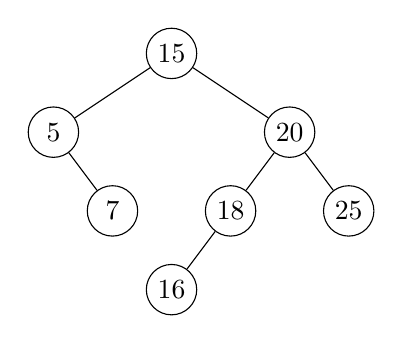
\begin{tikzpicture}[
	level distance=10mm,
	level 1/.style={sibling distance=30mm},
	level 2/.style={sibling distance=15mm}
]
\node{$15$}
child { node{$5$}
	child[missing]
	child { node{$7$} }
}
child { node{$20$}
	child { node{$18$}
		child { node{$16$} }
		child[missing]
	}
	child { node{$25$} }
};
\end{tikzpicture}

\subsection{Normal Tree}
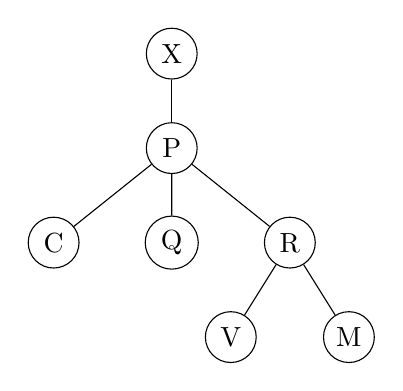
\begin{tikzpicture}[level distance=1.2cm]
\node{X}
child { node{P}
	child { node{C} }
	child { node{Q} }
	child { node{R}
		child { node{V} }
		child { node{M} }
	}
};
\end{tikzpicture}

\begin{forest}
for tree={circle,draw}
[, phantom, s sep = 1cm
	[1
		[2[3]]
		[4[5]]
		[6]
	]
]
\end{forest}

\subsection{Forest}
\begin{forest}
[, phantom, s sep = 1cm
[A
	[B [C] [D[E]] [F]]
	[G]]
[H
	[I]
	[J [K [L]]
	[M [N] [O]]]]
[P
	[Q] [R [S] [T]] [U] [V [W [X]] [Y]] [Z]]
]
\end{forest}

\end{document}
